\section{example}

男大学生自用99新latex模板。

\section{文献引用}

文献引用\cite[text]{example-bib}

\subsection{一级子目录}

ababab

\subsubsection{二级子目录}

ababab

\section{插入代码}


\subsection{直接嵌入代码块}

\begin{lstlisting}
    <dependency>
        <groupId>org.springframework.cloud</groupId>
        <artifactId>spring-cloud-starter-netflix-eureka-client</artifactId>
    </dependency>
\end{lstlisting}


\subsection{引用外部代码文件}

\lstinputlisting[
    style=file,
    label = {admin-service.java},
    caption = {\bf admin-service.java}
]{files/example/AdminServiceApplication.java}


\section{插入图片}

\subsection{使用{includegraphics}}


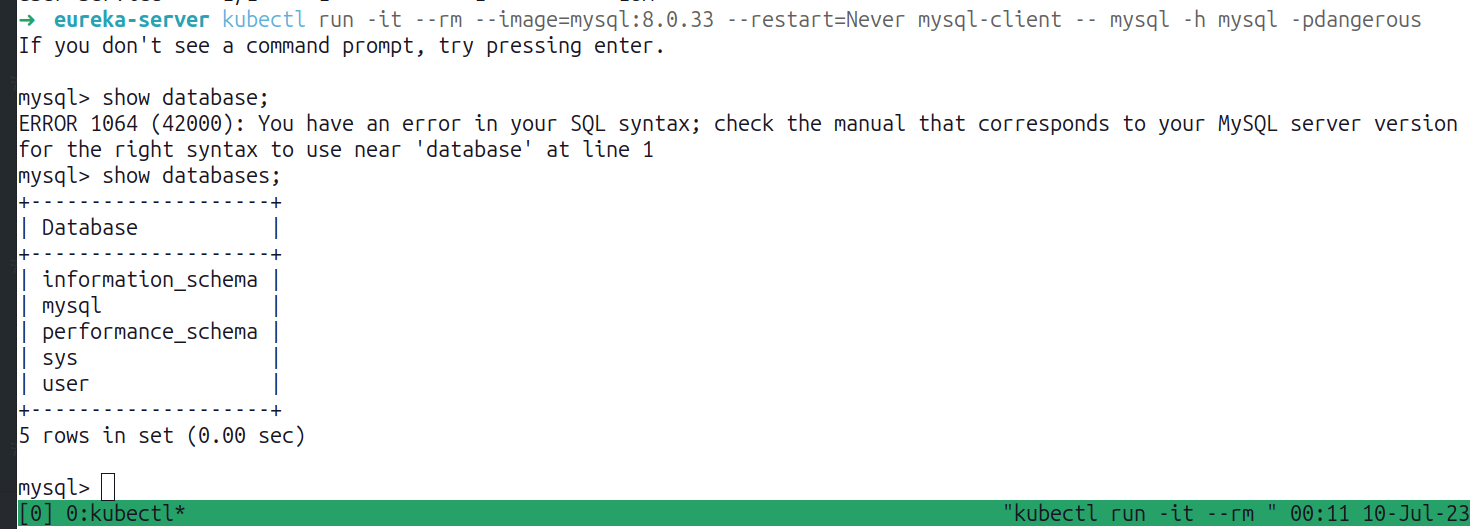
\includegraphics[width=0.9\linewidth]{figures/example.png}


\subsection{使用{subfig}}

subfig宏包:subfig宏包属于subfloat宏包系列,提供了创建并排子图的功能。
使用该宏包,您可以在一个浮动环境(如figure)中排列多个子图,并为每个子图添加标题和标签


subfigure宏包:subfigure宏包属于obsolete宏包系列,已经被推荐使用subfig或subcaption宏包来代替。
使用该宏包,您可以在一个浮动环境中排列多个子图,并为每个子图添加标题和标签。

引用示例:

Figure \ref{fig:subfig-example} has two sub-figures, fig. \ref{Fig.sub.1} \& \ref{Fig.sub.2}.

\begin{figure}
    \centering
    \subfloat[子图1\label{Fig.sub.1}]{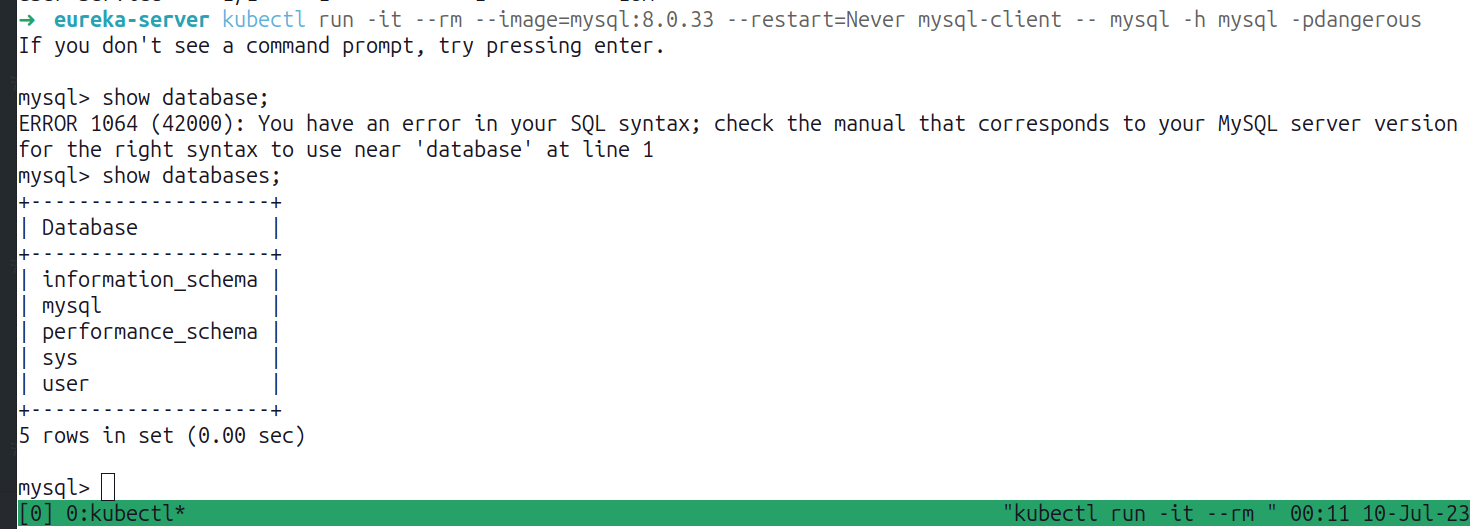
\includegraphics[width=0.3\textwidth]{figures/example.png}}
    \hfill
    \subfloat[子图2\label{Fig.sub.2}]{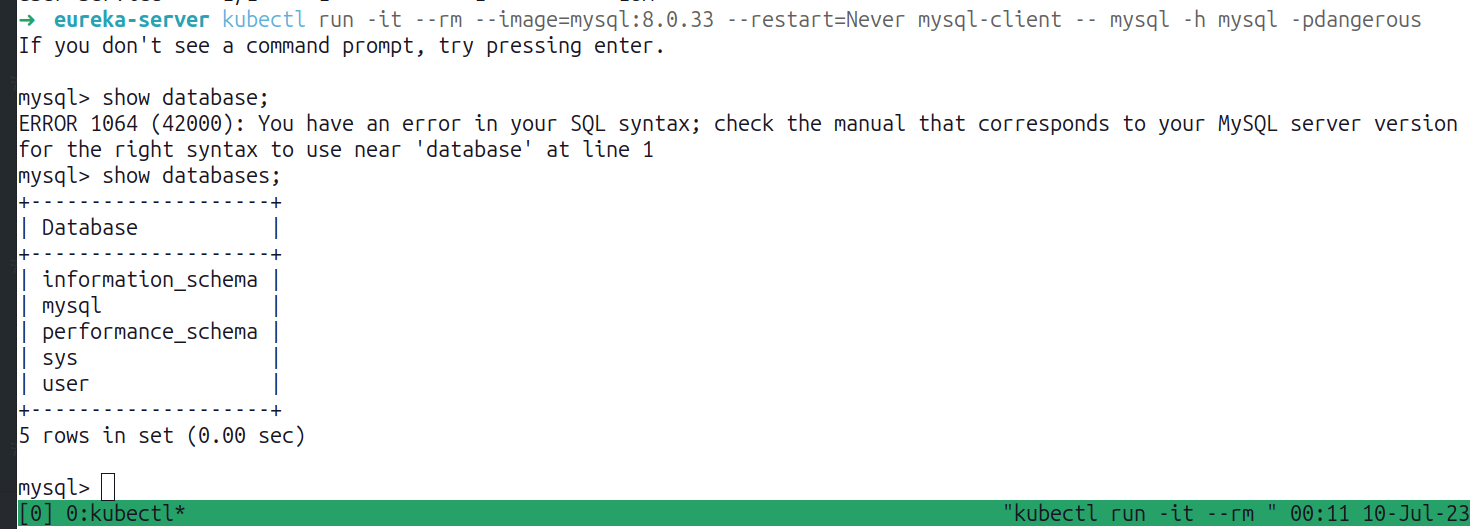
\includegraphics[width=0.3\textwidth]{figures/example.png}}
    \caption{多个子图示例}
    \label{fig:subfig-example}
\end{figure}

\section{伪代码}


\begin{algorithm}
    \caption{示例算法}\label{alg:example}
    \begin{algorithmic}[1]
    \Procedure{ExampleProcedure}{}
    \State $x \gets 0$
    \While{$x < 10$}
        \State $x \gets x + 1$
        \If{$x$ is even}
            \State \textbf{print} ``$x$ is even''
        \Else
            \State \textbf{print} ``$x$ is odd''
        \EndIf
    \EndWhile
    \EndProcedure
    \end{algorithmic}
\end{algorithm}
